\section{WebRTC}
\subsection{In General}
\begin{itemize}
  \item WebRTC for browser to browser communication.
  \item P2P, no server involved (-mostly. Server is needed to get the communication running).
  \item Real time communication (RTC) via API.
  \item Supported by Google, Microsoft, Mozilla, Opera, Apple
  \item Standard still not finalized
\end{itemize}

\subsubsection{Use Case}
\begin{itemize}
  \item Filling gap in the Web-Experience
  \begin{itemize}
    \item Video Chat $\rightarrow$ Google Hangouts Plugin, Flash, Java
    \item Multimedia / Conferences $\rightarrow$ Expensive, proprietary 3rd party apps
    \item Customer Service $\rightarrow$ Chat only, 3rd party plugins/apps
    \item Online Games $\rightarrow$ Flash
    \item Real-time Feeds $\rightarrow$ Proprietary software
    \item File Sharing $\rightarrow$ Requires Server / BitTorrent
  \end{itemize}
  \item WebRTC widely deployed, no client necessary!
  \item Used in WhatsApp, Facebook Messenger, whereby.com
  \item WebRTC forbids unencrypted communication
\end{itemize}

\subsubsection{Concerns}
\begin{itemize}
  \item Outdated documentation
  \item HTML browsers get bloated $\rightarrow$ Several GB RAM to open couple of tabs?
  \item WebRTC API could be simplified
  \item Security Concerns: Private IP / IP behind VPN, Tor? Not anymore!
  \item Complexity because of Security.
\end{itemize}

\subsubsection{Stream Control Transmission Protocol (SCTP)}
\paragraph{Pro}
\begin{itemize}
  \item SCTP Message-based (Like UDP, but reliable).
  \item Allows data to be divided into multiple streams.
  \item Syn cookies - SCTP uses a four-way handshake with a signed cookie.
  \item 32-bit end-to-end checksum (CRC32C).
  \item Multi-homing multiple IP addresses of endpoints.
\end{itemize}
\paragraph{Con}
\begin{itemize}
  \item Not widely used.
  \item If not used, tunneled over UDP.
\end{itemize}
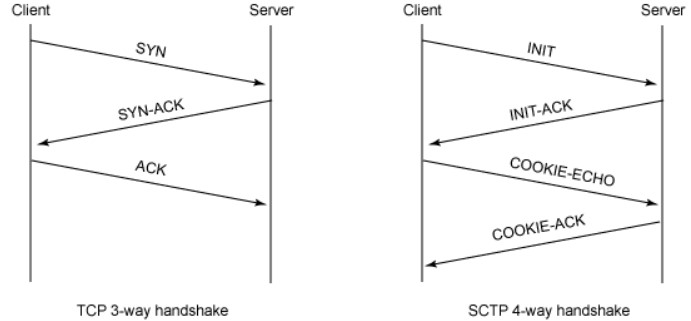
\includegraphics[width=\linewidth]{sctp.jpg}

\subsection{Introduction}
On the bright side: developer does not need to care about NAT.
Abstraction using STUN, ICE, TURN.

\subsubsection{STUN}
STUN: session traversal utilities for NAT (detect which kind of NAT).
Uses Tests to figured out if NAT is used and which.

\subsubsection{TURN}
traversal using relays around NAT
\begin{itemize}
  \item TURN always UDP server and the peer
  \item TURN client/server UDP, TCP/TLS
  \item UPnP / NAT-PMP setup by the browser optional?
  \item TURN is a relay extension for STUN
\end{itemize}
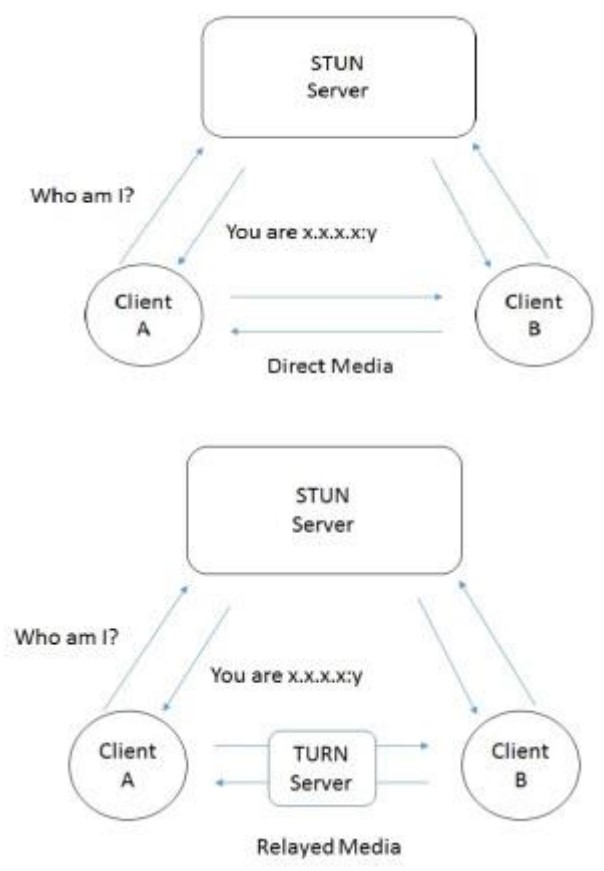
\includegraphics[width=\linewidth]{stun-turn.jpg}

\subsubsection{ICE}
Interactive Connectivity Establishment.\\
ICE works by exchanging a multiplicity of IP addresses and ports, which are then tested for connectivity by peer-to-peer connectivity checks.

\subsection{Connectivity}
Encryption is mandatory for all WebRTC components:
\begin{itemize}
  \item SRTP for Media, DTLS for Data, HTTPS for signaling
\end{itemize}
WebRTC is not a plugin.
\begin{itemize}
  \item Camera and microphone access must be granted explicitly
\end{itemize}
Once connection is established - easy API
\begin{itemize}
  \item RTCPeerConnection.send(``hallo'')
  \item RTCPeerConnection.onmessage = function \dots
\end{itemize}

\subsubsection{Triangle}
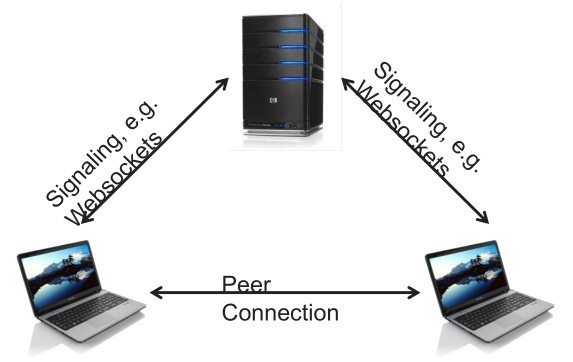
\includegraphics[width=\linewidth]{webrtc-triangle.jpg}

\subsubsection{Trapezoid}
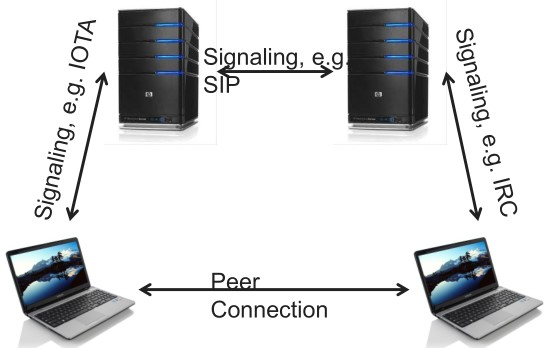
\includegraphics[width=\linewidth]{webrtc-trapezoid.jpg}

\subsubsection{Signaling PoC}
A proof-of-concept for WebRTC signaling using sound. Works with all devices that have microphone + speakers. Runs in the browser:\\
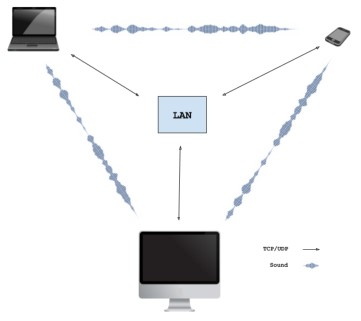
\includegraphics[width=\linewidth]{webrtc-signaling.jpg}

\subsection{Outlook}
\begin{itemize}
  \item Strong focus on VoIP.
  \item Fewer plugins (flash, java), fewer registrations
  \item New types of applications - Conferencing, gaming, P2P file sharing
  \item Object Real-Time Communications (ORTC) instead Session Description Protocol (SDP)
\end{itemize}
